%%% template.tex
%%%
%%% This LaTeX source document can be used as the basis for your technical
%%% paper or abstract. Intentionally stripped of annotation, the parameters
%%% and commands should be adjusted for your particular paper - title, 
%%% author, article DOI, etc.
%%% The accompanying ``template.annotated.tex'' provides copious annotation
%%% for the commands and parameters found in the source document. (The code
%%% is identical in ``template.tex'' and ``template.annotated.tex.'')

\documentclass[annual]{acmsiggraph}

\TOGonlineid{45678}
\TOGvolume{0}
\TOGnumber{0}
\TOGarticleDOI{1111111.2222222}
\TOGprojectURL{}
\TOGvideoURL{}
\TOGdataURL{}
\TOGcodeURL{}

\title{Mobile Depth from Focus and Applications}

\author{Naran Bayanbat\thanks{e-mail:jasonch@stanford.edu}\\Stanford University \and Jason Chen\thanks{e-mail:jasonch@stanford.edu} \\Stanford University \and Chun-Wei Lee\thanks{e-mail:jasonch@stanford.edu} \\Stanford University}
\pdfauthor{Naran Bayanbat, Jason Chen, Chun-Wei Lee}

\keywords{depth from focus, depth map, tablet, computational photography}

\begin{document}

 \teaser{
   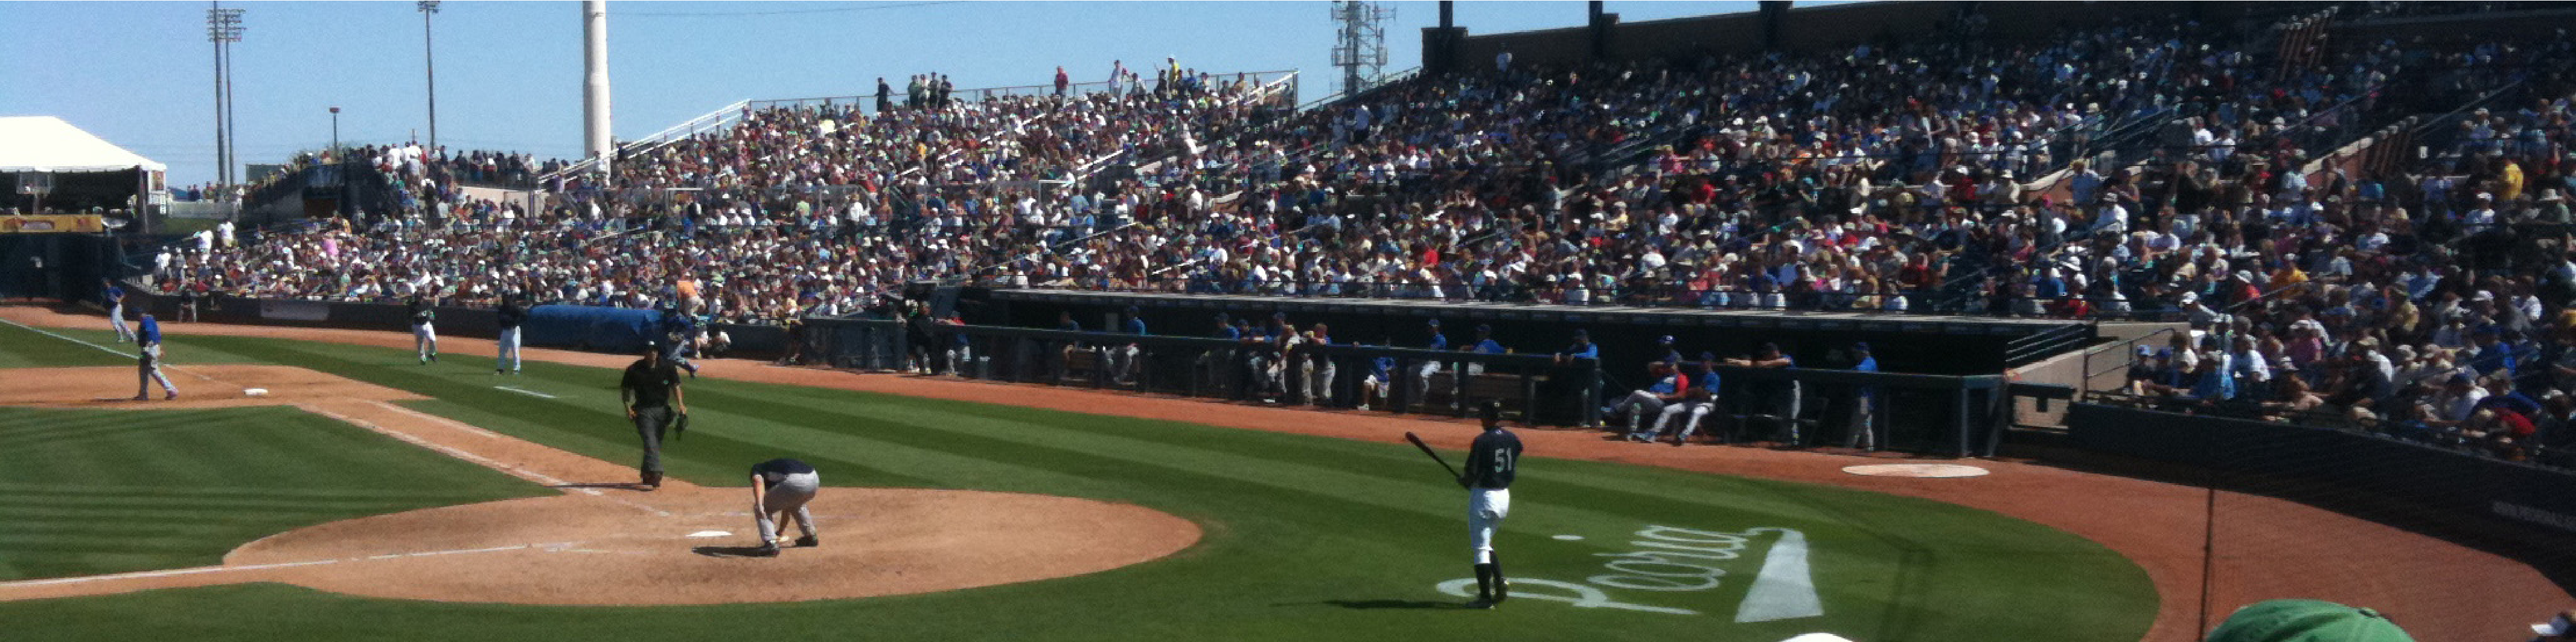
\includegraphics[height=1.5in]{images/sampleteaser}
   \caption{Spring Training 2009, Peoria, AZ.}
 }

\maketitle

\begin{abstract}
Depth information is crucial in providing scene understanding for many post-processing applications in computational photography. While depth maps can be easily obtained through stereo cameras or external devices such as infrared sensors, it is difficult in mobile photography because of hardware limitation. In this project, we will implement depth-by-focus, sweeping a single lens across various focus distances and composite an approximate depth map. The depth map will be improved by segmentation and bilateral filtering. We will then demonstrate the effectiveness of the technique by utilizaing the depth map and simulate light-field photography as well as synthetic depth of field.

\end{abstract}

\begin{CRcatlist}
  %\CRcat{I.3.3}{Computer Graphics}{Three-Dimensional Graphics and Realism}{Display Algorithms}
  %\CRcat{I.3.7}{Computer Graphics}{Three-Dimensional Graphics and Realism}{Radiosity};
\end{CRcatlist}

\keywordlist

%\TOGlinkslist

\copyrightspace

\section{Introduction}

Mobile devices have become the most common photography means, and they have presented a new set of opportunities and challenges for computational photography.  While many applications take advantage of these devices' location, accelerameter, and other meta data, the inherent hardware limitation on size computation power makes it worth revisiting prior works on computational photography to this application.  Specifically, since depth information is one of the most useful piece of scene understanding, we wish to demonstrate a mobile solution producing a depth map that assist in computational photography.  Since most mobile devices have only one camera (lens) and no active focusing equipment, we will attempt to implement depth from focus, approximating depth information from images captured at different depths. 

\section{Prior Work}

Depth from Focus is a technique that has been studied for decades \cite{Grossmann1987} and with numerous applications \cite{mobileRobot}.  It is useful 

\section{Results}

\section{Concolusions and Further Works}



\section*{Acknowledgements}


\bibliographystyle{acmsiggraph}
\bibliography{template}
\end{document}
